\title{Introdução a Filas e Pilhas}
\date{\today}
\frame{\titlepage}
% Slide 1: Conceito Detalhado de Filas
\begin{frame}[fragile]
  \frametitle{Conceito Detalhado de Filas}
  \begin{itemize}
    \item \textbf{Definição:} Uma fila é uma estrutura de dados linear que segue uma ordem específica para operações de adição e remoção de elementos. Essa ordem é baseada no princípio FIFO (First In, First Out), onde o primeiro elemento adicionado é o primeiro a ser removido.
    \item \textbf{Representação:} Visualmente, pode-se imaginar uma fila como uma linha de pessoas esperando para ser atendida em um banco, onde a primeira pessoa a chegar é a primeira a ser atendida.
    \item \textbf{Utilização:} Fundamental em situações que exigem manutenção da ordem original de eventos ou dados, como em sistemas operacionais para gerenciamento de processos e tarefas.
  \end{itemize}
\end{frame}

% Slide 2: Operações e Implementação de Filas
\begin{frame}[fragile]
  \frametitle{Operações e Implementação de Filas}
  \begin{itemize}
    \item \textbf{Operações Principais:}
      \begin{itemize}
        \item \textit{Enqueue (Inserir):} Adiciona um elemento ao final da fila.
        \item \textit{Dequeue (Remover):} Remove e retorna o elemento no início da fila.
        \item \textit{Peek/Front:} Retorna o elemento no início da fila sem removê-lo.
      \end{itemize}
    \item \textbf{Implementação:} Filas podem ser implementadas usando arrays ou listas ligadas. A escolha depende das necessidades específicas de desempenho e memória da aplicação.
  \end{itemize}
\end{frame}

% Slide 2: Operações e Implementação de Filas
\begin{frame}[fragile]
  \frametitle{Operações e Implementação de Filas}
  \begin{itemize}
    
    \item \textbf{Exemplo em Pseudocódigo:}
      \begin{verbatim}
      Enqueue(x):
        fila.append(x)
      
      Dequeue():
        if fila não está vazia:
          return fila.pop(0)
        else:
          return "Fila vazia"
      \end{verbatim}
  \end{itemize}
\end{frame}


% Slide: O Princípio FIFO e sua Aplicação em Filas
\begin{frame}[fragile]
  \frametitle{O Princípio FIFO e sua Aplicação em Filas}
  \begin{itemize}
    \item \textbf{Entendendo FIFO:} FIFO, sigla para First In, First Out, é um princípio fundamental de organização e processamento que estipula que o primeiro elemento a ser adicionado à estrutura será o primeiro a ser removido. Este conceito é essencial em muitas estruturas de dados, com destaque para as filas.
    \item \textbf{Importância em Filas:}
      \begin{itemize}
        \item Garante justiça e ordem na execução de tarefas ou no atendimento de solicitações, assegurando que não haja favorecimento ou atrasos indevidos.
        \item Facilita o planejamento e a previsão em sistemas de processamento, permitindo estimar o tempo de espera e alocar recursos de forma eficiente.
      \end{itemize}
  \end{itemize}
\end{frame}
\begin{frame}[fragile]
  \frametitle{O Princípio FIFO e sua Aplicação em Filas}
  \begin{itemize}
    \item \textbf{Aplicações Práticas:}
      \begin{itemize}
        \item \textit{Sistemas de Atendimento:} Em um restaurante com sistema de fila de espera, o cliente que chega primeiro, é atendido primeiro.
        \item \textit{Processamento de Tarefas:} Em um sistema operacional, processos em uma fila de execução são iniciados com base na sua ordem de chegada, garantindo um tratamento equitativo dos recursos do sistema.
      \end{itemize}
    \item \textbf{Conclusão:} O princípio FIFO é a espinha dorsal das filas, proporcionando uma base sólida para o desenvolvimento de algoritmos justos e eficientes em diversas áreas da computação e do cotidiano.
  \end{itemize}
\end{frame}


% Slide 3: Aplicação Prática de Filas
\begin{frame}[fragile]
  \frametitle{Aplicação Prática de Filas}
  \begin{itemize}
    \item \textbf{Gerenciamento de Tarefas em Sistemas Operacionais:} Um exemplo prático do uso de filas é no escalonamento de processos em sistemas operacionais. Processos são mantidos em uma fila, aguardando pela CPU. O agendador de tarefas seleciona processos da fila seguindo a ordem FIFO para execução.
    \item \textbf{Simulação de Cenário:}
      \begin{itemize}
        \item \textit{Situação:} Uma fila de impressão onde documentos são adicionados e impressos seguindo a ordem de chegada.
        \item \textit{Implementação:} A aplicação da fila garante que todos os documentos serão impressos na ordem correta, evitando conflitos e garantindo a equidade no uso da impressora.
      \end{itemize}
    \item \textbf{Benefício:} O uso de filas em tais sistemas assegura a transparência e eficiência no processamento de tarefas ou atendimento de solicitações.
  \end{itemize}
\end{frame}
% Slide: Aplicação de Filas em Sistemas de Gerenciamento de Filas
\begin{frame}[fragile]
  \frametitle{Aplicação de Filas em Sistemas de Gerenciamento de Filas}
  \begin{itemize}
    \item \textbf{Contexto:} Bancos, supermercados e repartições públicas onde o serviço é prestado com base na ordem de chegada dos clientes.
    \item \textbf{Implementação:} Utiliza-se uma fila para organizar os clientes de acordo com sua chegada, garantindo que o atendimento seja feito de forma justa e eficiente.
    \item \textbf{Benefícios:}
      \begin{itemize}
        \item Garantia de atendimento por ordem de chegada.
        \item Redução de conflitos e insatisfação dos clientes.
        \item Melhoria na previsibilidade e gestão do tempo de espera.
      \end{itemize}
    \item \textbf{Exemplo Prático:} Um sistema de senha em um banco, onde cada cliente retira uma senha ao entrar e é atendido quando seu número é chamado, seguindo estritamente a ordem de chegada.
  \end{itemize}
\end{frame}

% Slide: Aplicação de Filas no Processamento de Dados
\begin{frame}[fragile]
  \frametitle{Aplicação de Filas no Processamento de Dados}
  \begin{itemize}
    \item \textbf{Contexto:} Processamento e armazenamento temporário de dados em sistemas computacionais, como em streams de vídeo ou impressão de documentos.
    \item \textbf{Implementação:} Dados são colocados em uma fila, onde o primeiro a chegar será o primeiro a ser processado ou transmitido, garantindo a ordem correta de processamento.
    \item \textbf{Benefícios:}
      \begin{itemize}
        \item Mantém a integridade e a sequência dos dados durante o processamento.
        \item Facilita o gerenciamento de carga em sistemas de processamento, evitando sobrecarga e otimizando o uso dos recursos.
      \end{itemize}
    \item \textbf{Exemplo Prático:} Uma fila de impressão onde documentos enviados para a impressora são armazenados em uma fila e impressos na ordem em que foram recebidos.
  \end{itemize}
\end{frame}

% Slide: Aplicação de Filas no Controle de Tráfego de Redes
\begin{frame}[fragile]
  \frametitle{Aplicação de Filas no Controle de Tráfego de Redes}
  \begin{itemize}
    \item \textbf{Contexto:} Gerenciamento do fluxo de dados em redes de computadores, como na Internet ou em redes corporativas.
    \item \textbf{Implementação:} Filas são usadas para controlar o envio de pacotes de dados, garantindo que sejam enviados e recebidos em uma ordem lógica e eficiente.
    \item \textbf{Benefícios:}
      \begin{itemize}
        \item Priorização do tráfego, permitindo que pacotes críticos sejam processados antes.
        \item Prevenção de congestionamento na rede, gerenciando eficientemente o volume de dados.
      \end{itemize}
    \item \textbf{Exemplo Prático:} Em roteadores e switches, filas são utilizadas para ordenar pacotes de dados quando há mais dados chegando do que a capacidade de processamento ou largura de banda disponível, evitando a perda de dados importantes.
  \end{itemize}
\end{frame}

\end{frame}

% Slide 3: Introdução a Pilhas
% Slide: Conceito Detalhado de Pilhas
\begin{frame}[fragile]
  \frametitle{Conceito Detalhado de Pilhas}
  \begin{itemize}
    \item \textbf{Definição:} Pilhas são estruturas de dados abstratas que operam sob o princípio LIFO (Last In, First Out), onde o último elemento adicionado é o primeiro a ser removido.
    \item \textbf{Analogia Visual:} Imagine uma pilha de pratos em uma bandeja. O último prato colocado no topo é o primeiro a ser retirado quando necessário.
    \item \textbf{Características:}
      \begin{itemize}
        \item Simplicidade na adição e remoção de elementos, pois ocorrem no mesmo ponto.
        \item Facilidade na implementação em diversas linguagens de programação.
        \item Eficiência no gerenciamento de dados temporários, como históricos de navegação ou chamadas de funções.
      \end{itemize}
  \end{itemize}
\end{frame}

% Slide: Aplicações Práticas de Pilhas
\begin{frame}[fragile]
  \frametitle{Aplicações Práticas de Pilhas}
  \begin{itemize}
    \item \textbf{Execução de Chamadas de Função:} Pilhas são essenciais para gerenciar chamadas de função em programas, armazenando endereços de retorno e variáveis locais.
    \item \textbf{Avaliação de Expressões:} Utilizadas para avaliar expressões aritméticas e lógicas em notações como a postfix (polonesa inversa), facilitando a computação.
    \item \textbf{Navegação e Histórico:} Em interfaces de usuário, como navegadores web, pilhas ajudam a gerenciar o histórico de páginas visitadas, permitindo ao usuário retornar às páginas anteriores.
    \item \textbf{Desfazer Ações em Aplicativos:} Muitos softwares utilizam pilhas para permitir que os usuários desfaçam (undo) ações recentes de maneira ordenada e eficiente.
  \end{itemize}
\end{frame}

% Slide: Operações Básicas em Pilhas
\begin{frame}[fragile]
  \frametitle{Operações Básicas em Pilhas}
  \begin{itemize}
    \item \textbf{Push (Inserir):} Adiciona um elemento ao topo da pilha. É a operação que aumenta o tamanho da pilha, inserindo um novo elemento como o mais recente.
    \item \textbf{Pop (Remover):} Remove e retorna o elemento do topo da pilha. Esta operação diminui o tamanho da pilha, removendo o elemento que foi adicionado por último.
    \item \textbf{Peek/Top (Observar):} Retorna o elemento no topo da pilha sem removê-lo. Essencial para verificar o estado atual da pilha sem alterá-la.
  \end{itemize}
\end{frame}

\begin{frame}[fragile]
  \frametitle{Operações Básicas em Pilhas}
  \begin{itemize}
    \item \textbf{Exemplo em Pseudocódigo:}
    \small
    \begin{verbatim}
      push(x):
        pilha.add(x)

      pop():
        if pilha não está vazia:
          return pilha.remove(topo)
        else:
          return "Pilha vazia"

      peek():
        if pilha não está vazia:
          return pilha[topo]
        else:
          return "Pilha vazia"
      \end{verbatim}
  \end{itemize}
\end{frame}


% Slide 4: Exemplo de Aplicação de Pilhas
% Slide: Aplicação de Pilhas em Navegação na Web
\begin{frame}[fragile]
  \frametitle{Aplicação de Pilhas em Navegação na Web}
  \begin{itemize}
    \item \textbf{Contexto:} A navegação em sites na internet, onde cada página visitada é armazenada sequencialmente.
    \item \textbf{Implementação:} Uma pilha é usada para armazenar o histórico de páginas visitadas. Ao visitar uma nova página, a URL é "empilhada" no topo. Quando o usuário clica no botão de voltar, a página no topo da pilha é "desempilhada", e o navegador retorna à página anterior.
    \item \textbf{Vantagens:}
      \begin{itemize}
        \item Permite uma navegação intuitiva e eficiente entre as páginas visitadas.
        \item Facilita a implementação de recursos de histórico em navegadores web.
      \end{itemize}
    \item \textbf{Exemplo Prático:} Ao explorar links em uma página de notícias e depois utilizar o botão de voltar, o navegador usa uma pilha para determinar qual foi a última página visitada.
  \end{itemize}
\end{frame}

% Slide: Pilhas na Execução de Chamadas de Função
\begin{frame}[fragile]
  \frametitle{Pilhas na Execução de Chamadas de Função}
  \begin{itemize}
    \item \textbf{Contexto:} Programação de software, onde funções chamam outras funções durante a execução.
    \item \textbf{Implementação:} Cada chamada de função cria um novo quadro de pilha (stack frame) no topo da pilha, contendo informações como o ponto de retorno e variáveis locais. Quando uma função retorna, seu quadro de pilha é removido, retornando ao ponto de chamada.
    \item \textbf{Vantagens:}
      \begin{itemize}
        \item Garante a correta execução de funções e o retorno aos pontos de chamada apropriados.
        \item Facilita o rastreamento de chamadas de função e a depuração de programas.
      \end{itemize}
    \item \textbf{Exemplo Prático:} Em um programa que calcula fatorial, a função de fatorial chama a si mesma para cada valor decrementado até que atinja a base da recursão, utilizando uma pilha para controlar cada chamada.
  \end{itemize}
\end{frame}

% Slide: Pilhas na Avaliação de Expressões
\begin{frame}[fragile]
  \frametitle{Pilhas na Avaliação de Expressões}
  \begin{itemize}
    \item \textbf{Contexto:} Avaliação de expressões matemáticas, especialmente a conversão e avaliação de expressões infixas para postfixas (notação polonesa reversa).
    \item \textbf{Implementação:} Pilhas são usadas para armazenar operadores e operandos durante a conversão de expressões infixas para postfixas e durante a avaliação de expressões postfixas.
    \item \textbf{Vantagens:}
      \begin{itemize}
        \item Simplifica a computação ao eliminar a necessidade de considerar precedências de operadores fora da ordem.
        \item Torna mais eficiente a avaliação de expressões complexas em calculadoras e interpretadores de linguagem.
      \end{itemize}
    \item \textbf{Exemplo Prático:} Uma calculadora que avalia a expressão "3 + 4 * 2" primeiro converte para a forma postfixa "3 4 2 * +", depois avalia usando uma pilha para armazenar temporariamente os operandos e resultados parciais.
  \end{itemize}
\end{frame}
\begin{frame}[fragile]
  \frametitle{Jogo Torre de Hanoi}
  \begin{figure}
    \centering
    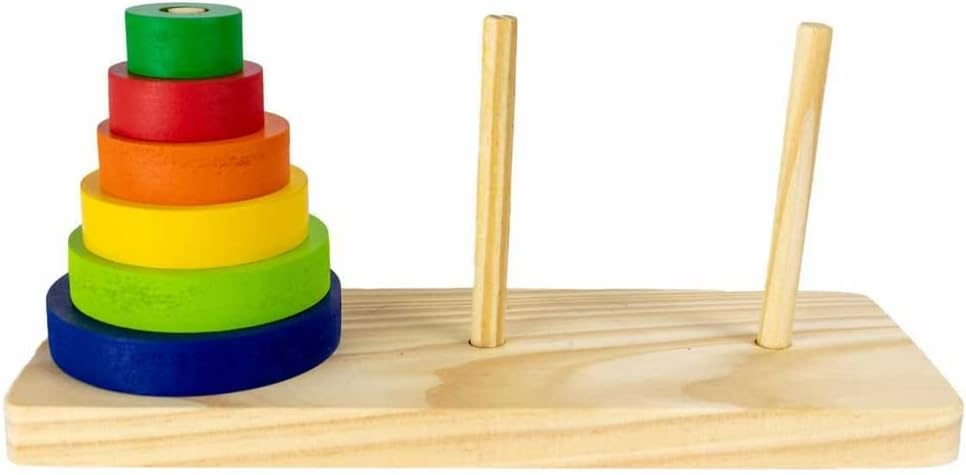
\includegraphics[width=0.8\textwidth]{assets/aula4-hanoi.jpg}
    \caption{Torre de Hanoi}
  \end{figure}
\end{frame}
% Slide: Introdução ao Problema da Torre de Hanoi
\begin{frame}[fragile]
  \frametitle{Introdução ao Problema da Torre de Hanoi}
  \begin{itemize}
    \item \textbf{Descrição do Problema:} O jogo da Torre de Hanoi consiste em três hastes e um número de discos de diferentes tamanhos que podem ser encaixados em qualquer haste. O objetivo é mover todos os discos de uma haste para outra, seguindo três regras simples:
      \begin{enumerate}
        \item Apenas um disco pode ser movido de cada vez.
        \item Cada movimento consiste em pegar o disco superior de uma das pilhas e colocá-lo no topo de outra pilha.
        \item Um disco maior não pode ser colocado sobre um disco menor.
      \end{enumerate}
    \item \textbf{Objetivo:} Mover todos os discos da haste origem para a haste destino, utilizando a haste auxiliar conforme necessário, com o menor número de movimentos possíveis.
  \end{itemize}
\end{frame}

% Slide: Algoritmo da Torre de Hanoi
\begin{frame}[fragile]
  \frametitle{Algoritmo da Torre de Hanoi}
  \begin{itemize}
    \item \textbf{Descrição do Algoritmo:} O algoritmo para resolver a Torre de Hanoi é um belo exemplo de aplicação de recursão. O processo pode ser descrito da seguinte forma:
      \begin{enumerate}
        \item Mover \(n - 1\) discos da haste origem para a haste auxiliar, usando a haste destino como intermediária.
        \item Mover o disco restante (o maior) para a haste destino.
        \item Mover os \(n - 1\) discos da haste auxiliar para a haste destino, usando a haste origem como intermediária.
      \end{enumerate}
    \item \textbf{Base da Recursão:} Quando resta apenas um disco, esse disco pode ser movido diretamente para a haste destino.
  \end{itemize}
\end{frame}

% Slide: Exemplo Prático do Algoritmo da Torre de Hanoi
\begin{frame}[fragile]
  \frametitle{Exemplo Prático do Algoritmo da Torre de Hanoi}
  \begin{itemize}
    \item \textbf{Cenário:} Considere um jogo da Torre de Hanoi com 3 discos na haste A (origem), com as hastes B (auxiliar) e C (destino) vazias.
    \item \textbf{Passos para Solução:}
      \begin{enumerate}
        \item Mova os dois primeiros discos para a haste B, usando C como intermediária.
        \item Mova o disco maior (o terceiro) para a haste C.
        \item Mova os dois discos de B para C, usando A como intermediária.
      \end{enumerate}
    \item \textbf{Resultado:} Todos os discos estão agora na haste C, na mesma ordem original, mas na haste destino, completando o jogo.
    \item \textbf{Nota:} Este procedimento minimiza o número total de movimentos necessários para resolver o jogo para qualquer número de discos.
  \end{itemize}
\end{frame}

\begin{frame}[fragile]
  \frametitle{Validação de Strings com Parênteses, Chaves e Colchetes}

  \textbf{Problema:} Dada uma string \(s\) contendo apenas os caracteres '(', ')', '{', '}', '[' e ']', determinar se a string de entrada é válida.

  \textbf{Critérios para uma string válida:}
  \begin{itemize}
    \item Parênteses abertos devem ser fechados pelo mesmo tipo de parênteses.
    \item Parênteses abertos devem ser fechados na ordem correta.
    \item Todo parêntese de fechamento tem um correspondente parêntese de abertura do mesmo tipo.
  \end{itemize}

  \tiny 
  referência: https://leetcode.com/problems/valid-parentheses/description/
\end{frame}

\begin{frame}[fragile]
  \frametitle{Validação de Strings com Parênteses, Chaves e Colchetes}

  \textbf{Exemplos:}
  \begin{itemize}
    \item Entrada: \(s = "()"\) \\
          Saída: verdadeiro
    \item Entrada: \(s = "()[]{}"\) \\
          Saída: verdadeiro
    \item Entrada: \(s = "(]"\) \\
          Saída: falso
  \end{itemize}

  \textbf{Restrições:}
  \begin{itemize}
    \item \(1 \leq \text{comprimento de } s \leq 10^4\)
    \item \(s\) consiste apenas de parênteses '()[]{}'.
  \end{itemize}
  \tiny 
  referência: https://leetcode.com/problems/valid-parentheses/description/
\end{frame}


\begin{frame}[fragile]
  \frametitle{Introdução à Notação Polonesa}
  
  \textbf{O que é Notação Polonesa (Notação Polonesa Reversa)?}
  \begin{itemize}
    \item Método de notação matemática onde cada operador segue todos os seus operandos.
    \item Remove a necessidade de parênteses para indicar a ordem das operações.
    \item Exemplo: A expressão convencional "3 + 4" é expressa como "3 4 +" na notação polonesa reversa.
  \end{itemize}
  
  \textbf{Vantagens da Notação Polonesa:}
  \begin{itemize}
    \item Simplifica a leitura e avaliação de expressões matemáticas.
    \item Elimina ambiguidades na ordem das operações sem o uso de parênteses.
  \end{itemize}
\end{frame}
\begin{frame}[fragile]
  \frametitle{Vantagens da Notação Polonesa Reversa}
  
  \textbf{Por que usar Notação Polonesa Reversa?}
  \begin{itemize}
    \item \textbf{Simplicidade de Avaliação:} Permite avaliação de expressões de forma sequencial, da esquerda para a direita.
    \item \textbf{Não Requer Parênteses:} A ordem de execução das operações é claramente definida pela posição dos operadores e operandos.
  \end{itemize}
  
  \textbf{Aplicações Práticas:}
  \begin{itemize}
    \item Amplamente utilizada em calculadoras científicas e em alguns tipos de computação.
    \item Facilita a implementação de algoritmos de avaliação de expressões em linguagens de programação.
  \end{itemize}
\end{frame}
\begin{frame}[fragile]
  \frametitle{A Importância das Pilhas na Notação Polonesa}
  
  \textbf{Como as Pilhas Facilitam a Avaliação:}
  \begin{itemize}
    \item Pilhas armazenam temporariamente os operandos durante a avaliação de expressões.
    \item Operadores aplicam-se aos elementos no topo da pilha; o resultado é recolocado na pilha.
  \end{itemize}
  
  \textbf{Benefícios do Uso de Pilhas:}
  \begin{itemize}
    \item Permite processamento direto e eficiente de expressões complexas.
    \item Essencial para a implementação de algoritmos de avaliação de expressões matemáticas em notação polonesa reversa.
  \end{itemize}
  
  \textbf{Conclusão:}
  O uso de pilhas é fundamental na notação polonesa reversa, oferecendo uma abordagem eficiente para o processamento de operações matemáticas.
\end{frame}
\begin{frame}[fragile]
  \frametitle{Exemplo de Cálculo em Notação Polonesa Reversa}

  \textbf{Expressão:} \(3\ 4\ +\ 2\ \ast\)

  \textbf{Objetivo:} Calcular a expressão usando notação polonesa reversa.
  
  \textbf{Processo:}

  \begin{enumerate}
    \item Iniciar com uma pilha vazia.
    \item Ler os elementos da expressão da esquerda para a direita:
      \begin{enumerate}
        \item Empilhar \(3\).
        \item Empilhar \(4\).
        \item Ler '+': desempilhar dois últimos números (\(4\) e \(3\)), somá-los (\(7\)), e empilhar o resultado (\(7\)).
        \item Empilhar \(2\).
        \item Ler '\(\ast\)': desempilhar dois últimos números (\(2\) e \(7\)), multiplicá-los (\(14\)), e empilhar o resultado (\(14\)).
      \end{enumerate}
    \item O resultado final (\(14\)) está no topo da pilha.
  \end{enumerate}

  \textbf{Resultado:} A expressão \(3\ 4\ +\ 2\ \ast\) é avaliada como \(14\), equivalente a \((3 + 4) \ast 2\) na notação convencional.
\end{frame}
\begin{frame}[fragile]
  \frametitle{Exemplo Complexo de Cálculo em Notação Polonesa Reversa}

  \textbf{Entrada:} tokens = ["10", "6", "9", "3", "+", "-11", "*", "/", "*", "17", "+", "5", "+"]

  \textbf{Objetivo:} Calcular a expressão usando notação polonesa reversa para obter o resultado 22.

  
\end{frame}

\begin{frame}[fragile]
  \frametitle{Exemplo Complexo de Cálculo em Notação Polonesa Reversa}



  \begin{enumerate}
    \item Expressão original em notação convencional: \(((10 \ast (6 / ((9 + 3) \ast -11))) + 17) + 5\)
    \item Simplificação passo a passo:
      \begin{enumerate}
        \item \(9 + 3 = 12\)
        \item \(12 \ast -11 = -132\)
        \item \(6 / -132 = 0\) (considerando divisão inteira)
        \item \(10 \ast 0 = 0\)
        \item \(0 + 17 = 17\)
        \item \(17 + 5 = 22\)
      \end{enumerate}
  \end{enumerate}

\end{frame}

\begin{frame}[fragile]
  \frametitle{Exemplo Complexo de Cálculo em Notação Polonesa Reversa}


  \begin{enumerate}
   
    \item Usando pilhas na notação polonesa reversa:
      \begin{enumerate}
        \item Empilha \(10, 6, 9, 3\), realiza \(9 + 3\) e empilha o resultado.
        \item Empilha \(-11\), realiza \(12 \ast -11\) e empilha o resultado.
        \item Realiza \(6 / -132\) (resultando em \(0\) com divisão inteira) e empilha.
        \item Empilha \(10\) e realiza \(10 \ast 0\), empilha o resultado.
        \item Empilha \(17\), realiza a adição com \(0\), e então empilha \(5\) e realiza a adição final.
      \end{enumerate}
    \item O resultado final no topo da pilha é \(22\).
  \end{enumerate}

  \textbf{Resultado:} A expressão complexa é avaliada como \(22\), demonstrando a eficácia da notação polonesa reversa e do uso de pilhas para avaliação de expressões matemáticas.
\end{frame}
